% --- Title Page ---
\newgeometry{left=3cm,right=3cm,top=2cm,bottom=2cm}

\begin{titlepage}
    \centering
    
    
\includegraphics[width=.3\textwidth]{Images/logo_uni.png}\\[1em]
    Fakultät für Sprach-, Literatur- und Kulturwissenschaften\\[1em]
    {\Large Research Proposal}\\[1em] 
    {Im Studiengang Englische Sprachwissenschaft}\\[1em]
    {Wintersemester 2025/26}

    \vspace{5cm}

    \textbf{\fontsize{16}{19}\selectfont Can AI Replace Traditional Textbooks?}\\[0.5em]
    \large \textbf{A Comparative Corpus Analysis of LLM-Generated vs. Textbook Example Sentences}

    \vspace*{\fill}

    \begin{flushleft}
        \begin{tabular}{ll}
            \textbf{Autor:} & Simon John \\
            \textbf{Matrikelnummer:} & 2175939 \\
            \textbf{Adresse:} & Wildbachweg 5, 93059 Regensburg \\ 
            \textbf{E-Mail:} & simon.john@stud.uni-regensburg.de \\ 
            \textbf{Studiengang:} & BA Englische Sprachwissenschaft \\ 
            \textbf{Abgabedatum:} & \today \\ %check
            \textbf{Gutachter:} & Dr.\ Thorsten Brato \\
        \end{tabular}
    \end{flushleft}
\end{titlepage}

\restoregeometry

% --- Front Matter ---
\newpage
\thispagestyle{empty}

% --- Table of Contents ---
\tableofcontents
\thispagestyle{empty}
\newpage

% --- List of Figures ---
\listoffigures
\thispagestyle{empty}
\newpage

\setcounter{page}{1} 

% --- Main Content ---
\section{Introduction}
Large Language Models (LLMs) like ChatGPT and Gemini are rapidly gaining recognition, even among the general public \parencite[see][]{mikhaylovArtificialIntelligencePublic2018}. Due to their vast capabilities in content generation, automated evaluation and workflow optimisation, Artificial Intelligence is increasingly being introduced into various private and public sectors. One prominent domain is the language learning classroom, redirecting attention from static learning materials, such as textbooks and novels, to dynamic, interactive tools. However, while there already is plenty of research on how AI handles student output, such as automated essay scoring or error correction, there is a noticeable gap in how we view these models as input providers.

This gap is significant because traditional ``Textbook English'' has long been criticised for being too stiff and unnatural. Traditional learning material tends to be syntactically strict and overly explicit, presenting a ``sanitised'' version of English that rarely matches how people actually speak. Here is where generative AI offers a promising alternative: the potential to simulate ``natural, casual'' English on demand. The question, however, is whether LLMs can truly recreate the nuances of authentic speech, or if they simply produce a statistically average imitation that is just as stiff and artificial as the textbooks they aim to replace.

While this study is motivated by Krashen's Input Hypothesis, which argues that language acquisition depends on exposure to high-quality, comprehensible input, this paper pivots to a data-driven approach. By utilising Corpus Linguistics methods, this proposal addresses the following research question: \textit{To what extent can Large Language Models (specifically Gemini Flash 2.5) generate linguistically distinct registers (formal, instructional, and casual) that quantitatively differ from human-authored textbook materials?} 

To answer this question, this study compiles a Natural Reference Corpus (NRC) from existing B1/B2 textbook materials and contrasts it with a Synthetic Control Corpus (SCC) generated via role prompting across three register conditions: formal workplace language (HIGH register: questions and professional contexts), instructional language (NEUTRAL register: imperatives, directions and rules), and casual conversational language (LOW register: statements in informal contexts). This design enables testing whether textbook English aligns most closely with formal, instructional, or casual native registers, or whether it represents a distinct pedagogical register unlike any of these.

\section{Theoretical Framework}
To effectively compare synthetic example sentences against traditional textbook materials, we need to choose concrete linguistic criteria that go beyond vague impressions of ``naturalness.'' This study grounds its analysis on the following criteria, building a robust framework that encapsulates three core areas of corpus linguistics: Register Theory, Idiomaticity and Complexity. Together, these criteria provide a basis that enables distinguishing between pedagogical language and authentic language usage.

\subsection{Register Theory: Defining ``Casualness''}
As \textcite{biber1988variation} argues, linguistic variation is never random and always functional. Linguistic features like pronouns, tense markers, or adverb classes tend to ``co-occur'' in texts, because they serve specific communicative functions \parencite[13]{biber1988variation}. By conducting factor analysis on various corpora, Biber identified certain ``dimensions'' of variation. For this study, Dimension 1: Involved vs. Informational Production \parencite[107]{biber1988variation} is a critical concept that will help to quantify the casualness of a text.

Textbooks are typically designed to transmit rules and vocabulary explicitly to ensure understandability. This design leans heavily toward the ``Informational Production'' pole. Casual language, the target of many language learners, however, sits at the other end of the spectrum: ``Involved Production''. Therefore, we can define casualness not by the presence of slang, but by a high frequency of features associated with involved production.

\subsubsection{Mood as an Operational Register Cue}

The methodological design of this study deliberately couples register prompts with grammatical mood (HIGH with interrogatives, NEUTRAL with imperatives, LOW with declaratives). This coupling requires explicit justification, because mood and register are not identical categories. Register describes recurring linguistic patterns in relation to communicative situation, whereas mood is a clause-level resource for interactional function \parencite{biber1988variation,biber1999longman,hallidayMatthiessenIntroductionFunctional2014}. In this proposal, mood is therefore treated as an operational cue that helps instantiate different communicative goals under controlled prompt conditions.

In this mapping, interrogatives are used to model formal workplace exchanges where clarification and information requests are frequent, imperatives are used to model instructional discourse with directive force, and declaratives are used to model casual narration and stance-sharing in everyday interaction \parencite{huddlestonPullumCambridge2002,quirkComprehensiveGrammar1985}. This does not claim that any single mood belongs exclusively to one register. Rather, it defines a controlled elicitation strategy that can induce contrasting communicative environments for subsequent corpus-based comparison.

If the AI effectively simulates a native casual register, the output text should be statistically marked by these three features:

\subsubsection{Interactive Pronouns}
    
The most obvious marker of involvement is the density of 1st and 2nd person pronouns (\textit{I, me, we, you}). Biber notes that a high frequency of these pronouns indicates ``interpersonal focus'' \parencite[102]{biber1988variation}. In contrast, textbooks tend to remove these interlocutors and focus on third-person objects or abstract nouns. \textit{I} and \textit{you} are much more frequent in conversation than other registers, because they act as an immediate anchor of discourse in direct interaction \parencite[333]{biber1999longman}.
    
\subsubsection{Situation-Dependent Reference}

Authentic conversations are rarely abstract. Most of the time, they refer to a specific time and place. This phenomenon is marked by adverbs of time and place like \textit{here, now, tomorrow, then} or \textit{yesterday}. Biber calls these ``situation-dependent'' references, because they rely strictly on the context for correct interpretation \parencite[37]{biber1988variation}. Textbook sentences, on the one hand, are often constructed to be ``timeless truths'' (e.g. \textit{``The bus leaves at 3 o'clock''}). Casual language, on the other hand, tends to be more immediate (e.g. \textit{``When did you get here?''}).
    
\subsubsection{Structural Reduction}

Casualness can also be characterised by speed and economy of expression. In corpora of spontaneous conversation, this often surfaces as \textit{structural reduction}: speakers compress forms that are predictable from context and rely on shared situational grounding. At the most visible level, this includes contractions (e.g. \textit{can't} vs. \textit{cannot}, \textit{I'm} vs. \textit{I am}), but reduction also extends to broader patterns such as complementiser deletion (e.g. omitting \textit{that} in \textit{``I hope you're well''}), ellipsis (dropping recoverable material in coordinated or adjacent clauses), and other shortened realisations that are common in spoken interaction \parencite{biber1999longman}.

For this proposal, structural reduction is relevant because textbook examples frequently avoid such reduced forms in favour of fully explicit, maximally transparent sentences. If the SCC-LOW is prompted to approximate a casual native register, it should therefore show a higher rate of these reductions (especially contractions and optional deletions) than the NRC, even when controlling for topic and sentence length.

\subsection{Idiomaticity} 

\subsubsection{The Open-Choice Principle}
    
To quantify authenticity beyond register analysis, this study uses Sinclair's \parencite*{sinclairCorpusConcordanceCollocation1991} two frameworks of language processing. In the Open-Choice Principle, a sentence is viewed as a series of empty slots (e.g. Subject + Verb + Object) that has to be filled by respective words fulfilling the grammatical conditions. Textbooks heavily rely on this framework to demonstrate grammatical rules in a straightforward, understandable way. This, however, often results in sentences that are syntactically perfect, but idiomatically unnatural (e.g. \textit{``I have entered the bus''}). 
    
\subsubsection{The Idiom Principle}

A speaker of a language has a large number of preconstructed phrases of a specific language at their disposal. They then proceed to take these loose chunks and combine them to form a new, cohesive sentence. Native speakers tend to think in these chunks to form sentences, rather than performing Open-Choice (e.g. \textit{``I got on the Bus''}).

This distinction is measurable by analyzing whether verbs are used literally (following the Open-Choice Principle) or idiomatically (following the Idiom Principle). Idiomatic usage includes phrasal verbs (e.g., \textit{put up with} meaning \textit{tolerate}), light-verb constructions (e.g., \textit{take responsibility}), and metaphorical extensions (e.g., \textit{run a company}). A statistically higher proportion of idiomatic usage in certain SCC registers would provide evidence that the AI can successfully mimic native phraseological patterns.

\subsection{Complexity}

A recurring issue in materials design is what one might call a ``paradox of simplification'': sentences are often simplified in order to help learners, but the result can on the contrary feel harder to process \parencite{spiroCognitiveFlexibility1992}. In this proposal, this is treated as a hypothesis about naturalness and learnability rather than an established claim. In particular, this study does not directly measure cognitive load. Instead, it explores whether corpus-based properties such as register, phraseology, and reduction correlate with differences in linguistic style that may relate to processing ease.

Accordingly, complexity is not treated as ``long sentences'' versus ``short sentences,'' but as a question of how input is packaged and how much interpretive work is required to understand the text.

To make this more concrete, this study draws on two perspectives that are commonly mentioned in second language acquisition (SLA) and educational psychology, namely Krashen's Input Hypothesis \parencite{krashenInputHypothesisIssues1985} and Sweller's Cognitive Load Theory \parencite{swellerCognitiveLoadProblem1988a}. These frameworks provide practical background needed to understand why differences in wording and information packaging might matter to the reader. They are not used to claim that any particular corpus feature (e.g. idiomatic density) reduces cognitive load.

\subsubsection{Krashen's Input Hypothesis}

Krashen's Input Hypothesis is often summarised with the formula $i+1$. The basic idea is that acquisition depends on exposure to input that is largely comprehensible at the learner's current level ($i$), while still containing some new material the learner is unfamiliar with (+1) \parencite{krashenInputHypothesisIssues1985}. This is most effectively achieved by immersion. For this study, this matters because the object of analysis is the example sentence. If sentences are the primary source of input in a textbook, then their register, phraseology and degree of contextualisation are not just stylistic features, but shape how easily learners can understand them.

At the same time, $i+1$ highlights a problem that is relevant for AI-generated text. A sentence can be authentic and still be too dense for B1--B2 learners if it relies on too many interacting unfamiliar elements (idioms, reduced forms, implications). In contrast, a sentence can be perfectly transparent, but so controlled that it no longer resembles how English is actually used. In other words, the question is not simply whether AI can generate ``native-like'' output, but whether it can be pushed towards a plausible $i+1$ zone for a given level.

\subsubsection{Sweller's Cognitive Load Theory}

Sweller's Cognitive Load Theory \parencite*{swellerCognitiveLoadProblem1988a} approaches the same problem from a different perspective. Sweller's hypothesis is based on the assumption that humans have a limited working memory, so learning is more effective when the material does not force learners to waste resources on avoidable difficulties. There is an important distinction between \textit{intrinsic load}, which comes from the inherent complexity of the content, and \textit{extraneous load}, which comes from how that content is presented. The presentation is particularly relevant for example sentences, because it is exactly where poorly chosen wording, weird information structure, or unnecessary redundancy can make an otherwise simple point harder than it needs to be.

In this proposal, CLT mainly functions as a motivation for focusing on presentation-related properties of sentences. However, this study does not test cognitive load directly. That is why any connection between observed patterns and processing effort is treated as suggestive rather than conclusive.

\section{Methodology}
This study uses a quantitative analysis based on corpora. The data collection and analysis are carried out with various Python scripts. For the AI-generated material, the scripts query \textit{Gemini Flash 2.5} via its API. For tokenisation and part-of-speech tagging, they rely on the \textit{Natural Language Toolkit} (NLTK) \parencite{birdKleinLoperNLP2009,loperBirdNLTK2002}. The goal is to keep the workflow transparent and easy to follow.

\subsection{Corpus Compilation}

This study aims to compare two different datasets: a Natural Reference Corpus (NRC) of authentic textbook English and a Synthetic Control Corpus (SCC) of LLM-generated sentences.

\subsubsection{Natural Reference Corpus (NRC)}

The NRC is compiled from the Textbook English Corpus (TEC), a specialised corpus assembled by Dr.\ Ellen Le Foll for investigating register variation in school EFL textbooks \parencite{leFoll2021b}. The TEC is a dataset containing pedagogical materials from published ESL/EFL textbooks \parencite{leFoll2021a}. Access to the TEC was granted through direct correspondence with the corpus compiler for academic research purposes.

Sampling procedure:
\begin{itemize}
    \item CEFR filtering: A subcorpus was created containing only B1/B2 level materials to match the proficiency target of the SCC.
    \item Target lemma extraction: Concordance searches were performed for the same 10 high-frequency polysemous verbs used in the SCC (\textit{take, make, hold, keep, break, run, drop, turn, see, look}).
    \item Verb-only filtering: All extracted sentences were processed through the same NLTK POS-tagging script described in Section~3.2.1 to collect only instances where the target lemma appears as a verb.
\end{itemize}

The NRC extraction and POS-filtering have been completed, yielding approximately 6200 sentences ready for semantic analysis. Upon approval, these sentences will be processed through the same \texttt{semantic\_analyzer.py} workflow used for the SCC.

The TEC contains materials from 33 different ESL/EFL textbooks published between 2006 and 2018 by seven major publishers (Oxford University Press, Cambridge University Press, Klett, Cornelsen, Nathan, Bordas, Richmond). The corpus represents both European markets (German \textit{Gymnasium} textbooks, French \textit{coll\`ege/lyc\'ee} materials) and international coursebooks, providing a representative sample of most pedagogical English from the 2000s--2010s.

The TEC represents ``traditional textbook English'' as it appears in published pedagogical materials. It functions as the baseline for evaluating whether LLM-generated examples differ systematically in register and idiomaticity. Unlike general corpora (e.g. BNC, COCA), the TEC specifically captures the pedagogical register that this study aims to compare against AI-generated alternatives.

\subsubsection{Synthetic Control Corpus (SCC)}

The current workflow is a pilot study built around a controlled list of ten high-frequency, polysemous target lemmas (\textit{take, make, hold, keep, break, run, drop, turn, see, look}). For each lemma, the script \texttt{scalable\_context\_generator.py} prompts Gemini Flash 2.5 via the API and automatically generates a set number of sentences under the following three conditions:

\begin{enumerate}
    \item {Register HIGH (Formal / Workplace; Questions)}
    \item {Register NEUTRAL (Direct / Instructions; Imperatives)}
    \item {Register LOW (Casual / Friends; Statements)}
\end{enumerate}

Each generated sentence is saved with metadata (\texttt{lemma}, \texttt{register}, \texttt{mood}) for register-based comparison.

\subsection{Computational Workflow}
Because textbook data is not structured and AI can produce occasional formatting mistakes, the processing follows a strict ETL workflow (Extract, Transform, Load) implemented in Python. In practice, this includes exporting the TEC sentence data from Sketch Engine and converting it into a consistent JSON/CSV format for further processing.

\subsubsection{POS-Tagging}
A central practical problem is that many of the target items are functionally ambiguous. For example, \textit{run} can appear as a noun (NN) as well as a verb (VB). If we simply searched for strings, we would keep irrelevant tokens (e.g. \textit{``a morning run''}) and distort the analysis.

To avoid this, the preprocessing step is handled by \texttt{pos\_tagger.py}. The script tokenises each sentence and applies the NLTK Averaged Perceptron Tagger. It then lemmatises tokens until a matching verb occurrence is found, and keeps the sentence only if it finds an occurrence whose lemma matches the \texttt{lemma} field in the JSON file (case-insensitive) and is tagged as a verb (i.e. a tag starting with \texttt{V}, such as VB, VBD, VBG, VBN, VBP, VBZ). This lemma-based matching ensures that inflected verb forms (e.g. \textit{runs}, \textit{ran}, \textit{running}) are counted as instances of the target lemma. Because the tagger operates on the same sentence JSON used throughout the workflow and performs basic NLTK checks before tagging, this step is reproducible and keeps the dataset consistent.

\subsubsection{Quantifying Idiomaticity: LLM as a Judge}
The current study analyses semantic behaviour directly by tagging each sentence-level occurrence of the target lemma as either \texttt{LITERAL} or \texttt{IDIOMATIC}. This is implemented as an \textit{LLM-as-a-judge} step: instead of hand-coding every single step here (e.g. regex patterns for verb+particle sequences), Gemini is used to make a constrained semantic decision for each sentence \parencite{zhengJudgingLLMas2023}. This is appropriate here because idiomaticity is not limited to particle verbs. It is even more helpful, because many de-lexicalised or metaphorical uses (e.g. \textit{run a company}) would be missed by standard regex rules.

This tagging is performed by \texttt{semantic\_analyzer.py}, which sends small chunks of sentences to Gemini and requests a strict JSON array of labels. The dependent variable is therefore \texttt{Usage\_Category} (\texttt{LITERAL} vs. \texttt{IDIOMATIC}), and the key grouping variable is \texttt{Register} (HIGH / NEUTRAL / LOW).

\subsection{Statistical Analysis}
The primary statistical test is a Chi-Square test of independence ($\chi^2$) to check whether \texttt{Register} (HIGH / NEUTRAL / LOW) and \texttt{Usage\_Category} (LITERAL / IDIOMATIC) are independent \parencite{agrestiCategoricalData2012}. The significance level is set to $\alpha = 0.05$.

Because the $\chi^2$ test assumes sufficiently large frequencies, low counts in some lemma\,$\times$\,register\,$\times$\,category combinations may not be accurate. Therefore, Fisher's Exact Test \parencite*{Fisher1992exacttest} will additionally be used as to check small expected frequencies.

The script \texttt{visualizer.py} additionally produces the two plots included in the appendix: an aggregate stacked bar chart by register and a per-lemma heatmap of \texttt{IDIOMATIC} rates.

\section{Limitations}

\subsection{Model Bias (Technical)}
This study uses Gemini 2.5 Flash for both data generation and semantic evaluation for API cost efficiency. While the model is great for high-volume processing, ``Flash'' models are optimised for latency rather than deep reasoning. That is why the model may show a ``simplicity bias,'' potentially under-reporting complex idiomatic usage compared to larger reasoning models (e.g., Claude Opus 4.5 or GPT-5.2). Future iterations of this study could use a multi-LLM design to cross-validate results across different models.

\subsection{Proxy Measures (Methodological)}
Furthermore, the operationalisation of linguistic variables relies on proxy measures. For example, while Section~2.1.3 defines ``structural reduction'' briefly (including contractions and ellipsis), the current workflow quantifies it via a simple apostrophe-based contraction count. This count does not distinguish between clitics (e.g., ``I'm'') and possessive markers (e.g., ``John's''), and it may also count apostrophes occurring inside quoted material. Ellipsis is not included in the present implementation.

The study couples register with grammatical mood (HIGH = Questions, NEUTRAL = Imperatives, LOW = Statements). This means that any observed differences in idiomaticity cannot be cleanly attributed to register (formal vs. casual) because they may instead be caused by mood-specific syntax (e.g. interrogatives often introduce auxiliaries such as \textit{could} or \textit{will} in subject-auxiliary inversion \parencite{huddlestonPullumCambridge2002,quirkComprehensiveGrammar1985}). A more robust design would decouple register and mood by crossing conditions (e.g. HIGH-Q workplace questions, HIGH-S workplace statements, LOW-Q casual questions, LOW-S casual statements). This would increase corpus size but allow separating register effects from mood effects.

\subsection{Model Self-Preference}
A potential concern arises from the ``LLM-as-a-judge'' methodology. As the same model family (Gemini) is used to both generate the Synthetic Control Corpus and classify its semantic usage, there is a risk of self-preference bias. The model may be inclined to rate its own generations as contextually appropriate. Future research should employ an independent ``judge'' model to ensure independence during the evaluation process.

\subsection{Corpus Representativeness}

The NRC derived from an established pedagogical corpus (TEC), represents a specific subset of textbook English: materials explicitly designed for B1/B2 learners. This has two implications.

First, the findings may not generalise to other CEFR levels. A1/A2 materials may show even higher explicitness (lower idiomaticity), while C1/C2 materials may contain more authentic registers.

Second, the TEC compilation date range (2006--2018) means the NRC reflects textbook design practices from that period. Le Foll's \parencite*{leFoll2021b} analysis of the TEC found that textbook English shows distinct register characteristics compared to general English corpora, particularly in its pedagogical framing and explicit grammatical structures. Therefore, if current ELT materials (2020--2025) show narrower gaps between textbook and authentic language, this would support H2 (Corpus-Informed Pedagogy Hypothesis) and suggest that LLMs are converging with an already-shifting policy of the design of learning material. On the other hand, if the 2006--2018 TEC materials already show substantial idiomaticity, this would challenge the assumption that textbooks avoid phraseological variation.

Despite these challenges, the B1/B2 focus is methodologically appropriate because this proficiency band represents the majority of adult ESL learners and is the primary target for intermediate textbooks where the difference between ``teachability'' and ``authenticity'' has arguably the most impact on the learner.

\section{Expected Outcomes and Alternative Hypotheses}

Based on the theoretical framework, three outcomes are possible:

\textit{H1 (Pedagogical Simplification Hypothesis):} The NRC will show significantly higher \texttt{LITERAL} usage than all SCC registers, reflecting textbooks' reliance on the Open-Choice Principle \parencite{sinclairCorpusConcordanceCollocation1991}. If confirmed, this would suggest LLM-generated examples could complement textbooks by providing more idiomatic, register-appropriate input at the same CEFR level.

\textit{H2 (Corpus-Informed Pedagogy Hypothesis):} The NRC will show pattern similar to SCC-NEUTRAL, indicating that modern textbooks already incorporate authentic phraseology. This would suggest that LLMs offer limited added value for idiomaticity.

\textit{H3 (Controlled Idiomaticity Hypothesis):} The NRC will show selective idiomatic usage (e.g. high-frequency phrasal verbs such as \textit{take off}) but avoid lower-frequency or colloquial idioms. This would indicate a pedagogical middle ground that neither purely literal examples nor fully native-like registers capture.

Preliminary $\chi^2$ analysis (Section~3.3) will determine which hypothesis the data supports.

\section{Conclusion}
\label{sec:conclusion}

This proposal asks a practical question: can an LLM be pushed to generate example sentences that are not only well-formed, but also measurably different in register? Building on register variation research, the study compares LLM output to sentences already used in ESL/EFL textbooks and tests whether the distributions of semantic usage differ across conditions.

Rather than relying on intuition about what ``sounds natural,'' the analysis treats each sentence as a unit and evaluates whether target-lemma patterns shift between \texttt{LITERAL} and \texttt{IDIOMATIC} realisations in ways consistent with existing frameworks of language use \parencite{sinclairCorpusConcordanceCollocation1991}. In practice, this matters because input quality is crucial to learnability. Register-appropriate, idiomatic but comprehensible examples are more likely to support acquisition without adding unnecessary processing load \parencite{krashenInputHypothesisIssues1985,swellerCognitiveLoadProblem1988a}.

The NRC has been compiled from the TEC and is ready for analysis. Upon approval, the NRC sentences will be semantically tagged using the validated SCC pipeline, and the resulting distributions will be compared against the SCC data to test the three competing hypotheses. Results will be reported in the final thesis.

% --- References ---
\newpage
\section*{References}
\addcontentsline{toc}{section}{References}
\printbibliography[heading=none]

% --- Documentation of AI Tools Used ---
\newpage
\section*{Documentation of AI Tools Used}
\addcontentsline{toc}{section}{Documentation of AI Tools Used}

In accordance with Section 3.3 of the \textit{Guidelines for Writing Term papers, Reports and Theses in English Linguistics at the University of Regensburg}, the use of generative Artificial Intelligence (specifically Google Gemini 2.5 Flash, Gemini Advanced, and Grammarly) in this thesis is documented as follows:

\begin{itemize}
    \item \textbf{Ideation and Brainstorming:} LLMs (Gemini) were utilized as a sparring partner for generating initial ideas, structural outlining, and brainstorming the theoretical framework.
    \item \textbf{Proofreading and Language Revision:} Grammarly was employed exclusively for post-drafting orthographic, grammatical, and stylistic proofreading. The tool was used solely to flag mechanical errors and improve readability, not to generate original academic content or arguments.
    \item \textbf{Code and Formatting Assistance:} AI was used as a technical assistant to troubleshoot Python data-processing scripts (e.g., pandas, NLTK) and to assist with LaTeX typesetting.
    \item \textbf{Methodological Instrument (Corpus Generation \& Semantic Classification):} The Gemini API was systematically employed as a research tool to generate the Synthetic Control Corpus (SCC) and act as an automated "LLM-as-a-judge" for semantic classification. This usage constitutes the primary object of investigation in this comparative corpus analysis and is thoroughly detailed and validated in the Methodology (Chapter 3).
\end{itemize}

\vspace{1em}
\noindent In strict adherence to departmental guidelines, generative AI was \textbf{not} used for generating entire texts or text passages of this thesis. All written text, theoretical interpretations, and final academic conclusions are entirely my own original work.

% --- Plagiarism Statement ---
\newpage
\section*{Plagiarism Statement}
\addcontentsline{toc}{section}{Plagiarism Statement}

I hereby declare that I have independently written the present work and have not used any aids other than those indicated. Any passages taken verbatim or in substance from other works (including those from electronic databases or the internet) have been clearly marked as such, with proper citation according to academic referencing rules. This declaration also applies to any visual representations, tables, maps, and drawings included in the work. I know any deception will be penalised according to the applicable study and examination regulations.

A Large Language Model (LLM) was used during the ideation process; however, the text and ideas presented are my own unless otherwise specified.

\vspace{2.5\baselineskip}
\noindent
\includegraphics[height=2cm]{Images/signature.png}\\
Regensburg, \today

% --- Appendix ---
\newpage
\appendix

\section{TEC Source Textbooks (B1/B2 Subset)}
\label{sec:tec-textbooks}

The following textbook titles (B1/B2-level subset) were included in the TEC-derived NRC sample:

\begin{itemize}
    \item \textit{Achievers B1} (2015)
    \item \textit{Achievers B1+} (2015)
    \item \textit{Achievers B2} (2015)
    \item \textit{Hi there!} 3e, Niveau A2--B1 (2015)
    \item \textit{Join the Team} 4e, A2--B1 (2012)
    \item \textit{Join the Team} 3e, A2--B1 (2013)
    \item \textit{New Missions} 2de, A2--B1 (2014)
    \item \textit{Solutions Pre-Intermediate} (2017)
    \item \textit{Solutions Intermediate} (2016)
    \item \textit{Solutions Intermediate Plus} (2017)
\end{itemize}

\newpage
\section{Preliminary Results (SCC Pilot Study)}

\noindent The following results are based on the AI-generated Synthetic Control Corpus (SCC) pilot data only. The Natural Reference Corpus (NRC) has been compiled and is ready for analysis. Semantic tagging and statistical comparison will be conducted upon approval.

\begin{figure}[H]
    \centering
    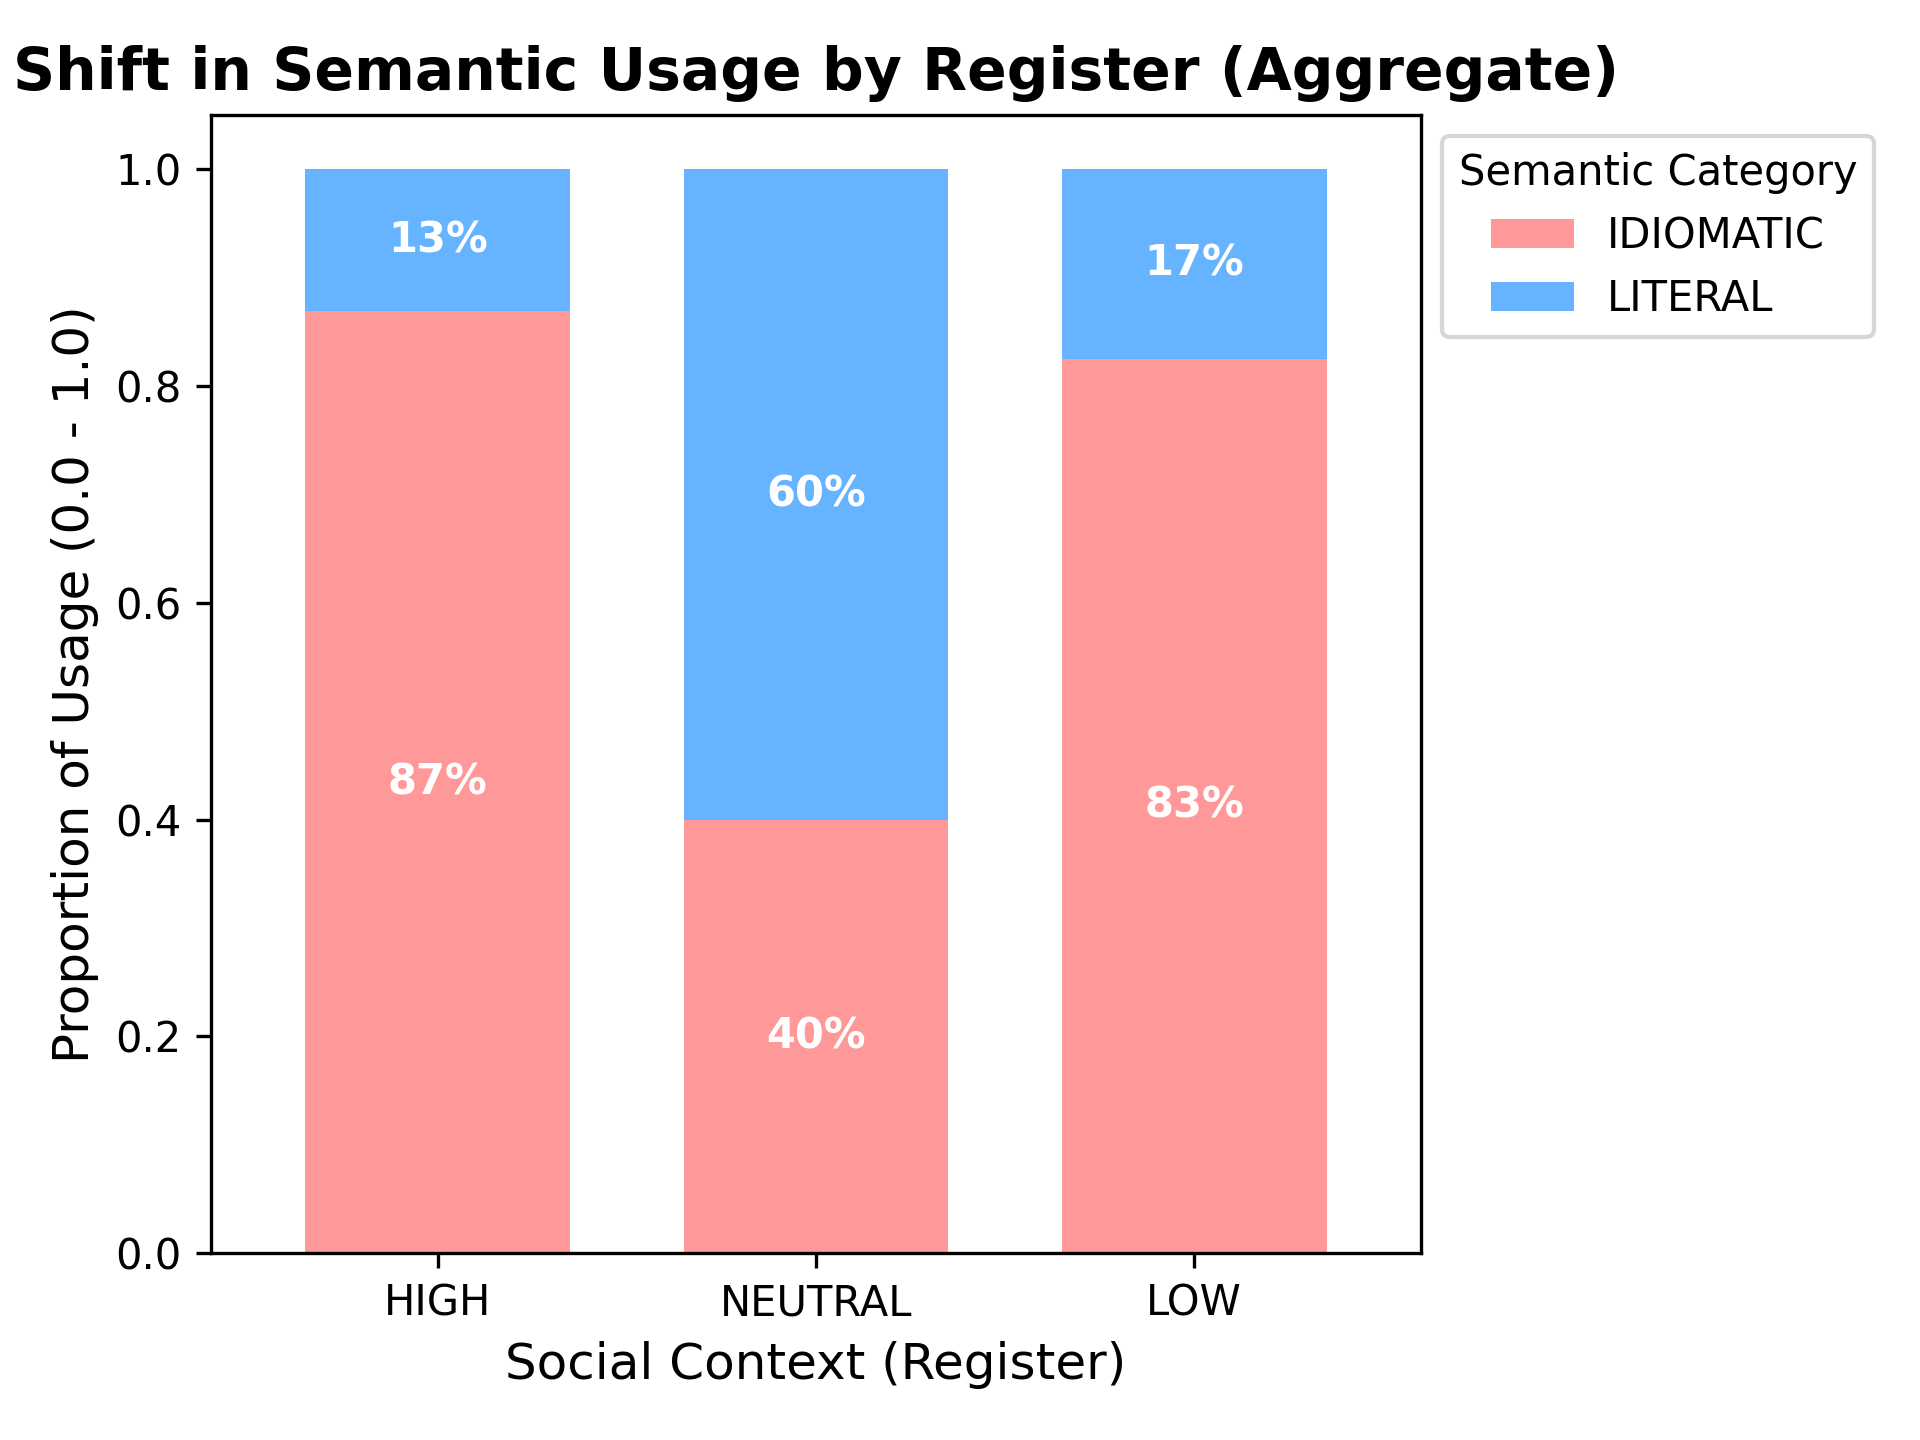
\includegraphics[width=\textwidth]{Images/results_aggregate_chart.png}
    \caption{Aggregate proportion of \texttt{LITERAL} vs. \texttt{IDIOMATIC} usages by register (SCC pilot data).}
    \label{fig:results-aggregate-appendix}
\end{figure}

\vspace{-0.75\baselineskip}
\begin{figure}[H]
    \centering
    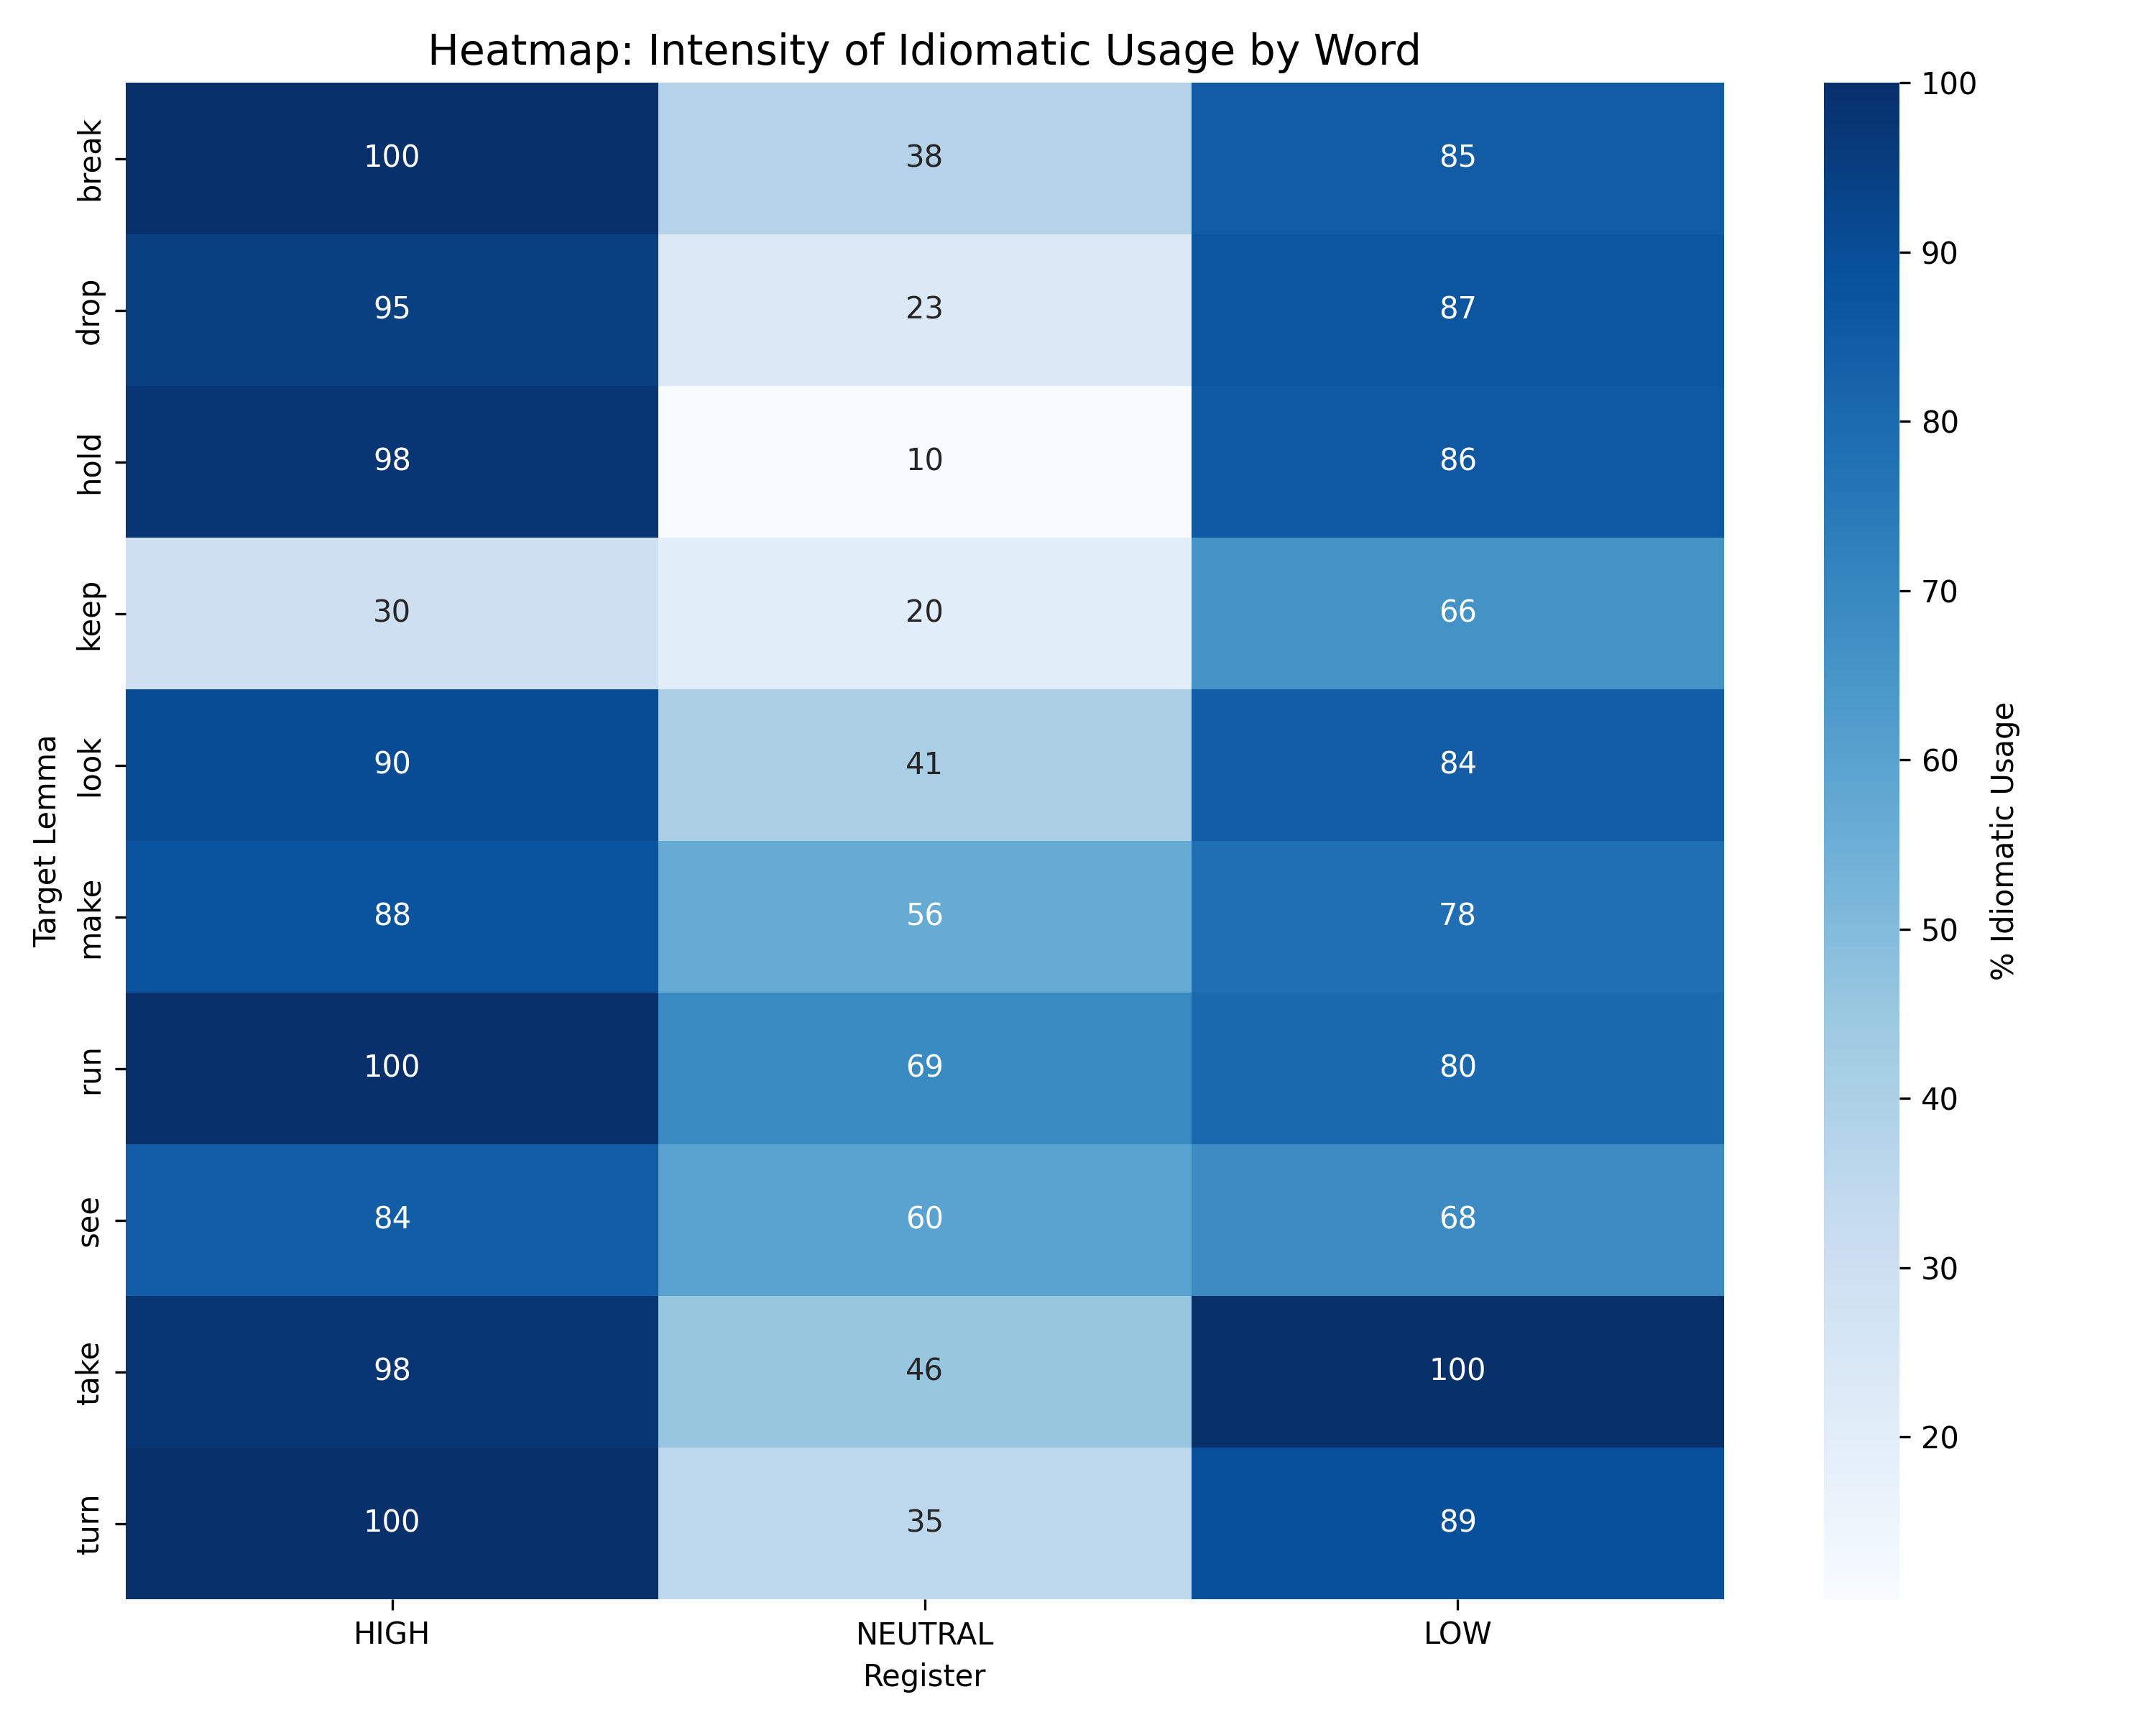
\includegraphics[width=\textwidth]{Images/results_heatmap.png}
    \caption{Per-lemma heatmap of \texttt{IDIOMATIC} usage rates by register (SCC pilot data).}
    \label{fig:results-heatmap-appendix}
\end{figure}

\subsection{Short Interpretation: \textit{run}}
In the pilot data, \textit{run} is classified as 100\% \texttt{IDIOMATIC} in the HIGH register. This aligns with the ``Workplace/Professional'' prompt condition: in professional contexts, \textit{run} is typically used metaphorically (e.g. \textit{run a meeting}, \textit{run tests}, \textit{run a project}) rather than to describe physical motion. For example, the synthetic HIGH-register sentence ``Could you confirm if the new software will run efficiently on older systems?'' uses \textit{run} in the sense of ``operate/function,'' i.e. a non-literal (de-lexicalised) usage.

In the LOW register, \textit{run} is 80\% \texttt{IDIOMATIC}. This is expected because casual contexts plausibly include literal movement (e.g. \textit{I ran to the store}), increasing the share of \texttt{LITERAL} uses.

\subsection{Short Interpretation: \textit{take}}
The word \textit{take} shows a V-shaped pattern. In HIGH (formal register), 98\% of uses are \texttt{IDIOMATIC}, light-verb constructions like \textit{take responsibility} or \textit{take measures}, where \textit{take} carries minimal semantic weight (e.g. from the SCC: ``Might this project take an unexpected turn given the new market analysis?''). In NEUTRAL (instructions), this drops to 46\%, with \textit{take} used literally (\textit{Take an exit}, \textit{Take one tablet}). In LOW (casual), idiomaticity rises back to 100\%, because of phrasal verbs like \textit{take off} or \textit{take it easy} (e.g. from the SCC: ``She always takes her time getting ready, it's so annoying.'').

In the SCC pilot, both formal and casual registers show high idiomaticity, while the AI-generated instructional register shows substantially lower idiomaticity. This pattern raises the question whether actual textbook-style examples similarly suppress idiomatic usage. This will be tested against the NRC in the full analysis.

\clearpage
\section{Python Code Documentation}

\noindent\textbf{Note:} The code shown below uses simplified file paths for readability. The actual repository implementation uses organized directories (\texttt{outputs/}, \texttt{data/}, \texttt{src/}) and environment variables for API keys. See the GitHub repository for the actual code, dataset and version history. 

\texttt{github.com/Eidolom/llm-corpus-generation-analysis}

\subsection{debug.py}
\lstinputlisting[language=Python]{code/debug.py}

\subsection{scalable\_context\_generator.py}
\lstinputlisting[language=Python]{code/scalable_context_generator.py}

\subsection{target\_words.txt}
\lstinputlisting[language={}]{code/target_words.txt}

\subsection{sketch\_engine\_converter\_nltk.py}
\lstinputlisting[language=Python]{code/nltk_sketch_engine_converter.py}

\subsection{pos\_tagger.py}
\lstinputlisting[language=Python]{code/pos_tagger.py}

\subsection{semantic\_analyzer.py}
\lstinputlisting[language=Python]{code/semantic_analyzer.py}

\subsection{visualizer.py}
\lstinputlisting[language=Python]{code/visualizer.py
}